\section{Introduction}\label{intro}

In the past decade, the use of smartphones has grown significantly among consumers.
According to a recent report~\cite{Ericsson}, there are 3.4 billion smartphone users worldwide,
and the accumulated mobile data traffic has reached 120 exabytes in 2015.
One critical reason for this explosive growth is the popularity of smartphone apps,
such as those served by Google Play and Apple Store,
whose number has exceeded 1.5 million by July 2015~\cite{Statista}.
It is estimated that people spend as much as 30 hours monthly on these apps on average,
a growth of over 65 percent compared to 2013~\cite{Nielsen}.

Consequently, recent research has invested considerable effort to understand smartphone app usage behavior,
as such understandings can help app developers and mobile advertisers tremendously~\cite{xu2011identifying,yang2015characterizing}.
In the previous work, both temporal patterns (\eg individual app usage histories) and
spatial patterns (\eg location contexts) have been extensively studied~\cite{meng2014analyzing}.
Their results have enabled novel applications,
such as smartphone app launching prediction services~\cite{yan2012fast}.

In this paper, we focus on one less investigated feature, user mobility,
and investigate how this feature correlates with the usage patterns of smartphone app users.
Understanding such correlations, if any, could provide useful contextual information
for relevant and accurate app recommendation and ad delivery.
For example, if we find out hiking hobbyists use certain apps considerably more often,
then such apps may be more useful venues for ad delivery for equipment makers for hiking activities.

Unfortunately, previous work on this topic has only investigated this problem in highly limited and controlled contexts,
and by taking account into the usage history of a small set of users.
For example, a few works have addressed the problem of transportation mode inference,
where the goal is to find out whether a user is riding a bus or taking a taxi, among other possibilities.
Such work usually assumes that additional hardware (\eg GPS, sensors) is available,
and is carried out for a small group of users in controlled experiments~\cite{6958169, 6450942, zheng2010understanding, biljecki2013transportation, stenneth2011transportation, 5283030, 6460199, Reddy:2010:UMP:1689239.1689243}.
Later work suggested that it may be possible to use cell tower communications to monitor users' mobility indirectly~\cite{rose2006mobile},
where efforts have been focusing on inferring users' trajectories~\cite{Alsolami2012Auth,jiang2013review}
or transportation mode~\cite{wang2010transportation,bekhor2015investigation} only using cell-phone traces
(\eg Call Detail Records, handover data) that do not directly contain location information.
Such approaches are more scalable, as they do not require additional hardware resources and better respect users' privacy.
The limitations of these approaches, however, are that they are usually small-scale by nature, and
usually has ground-truth data collected for a user as validation methods for their approaches.

Our work is following this latter line of research of using large-scale cell-phone tower traces.
However, our dataset and the corresponding methodology are significantly different.
First, our dataset consists of a truly large population,
where we have access to mobile data access histories of millions of users in three cities that cover thousands of square miles.
The number of users is perhaps more than the population of certain countries in the world.
Second, due to privacy concerns, the dataset is fundamentally coarse-grained,
meaning that we do not, and can not, collect the ground truth information for these millions of users.
Therefore, novel data processing methods are urgently needed.
Finally, our research goals are to reveal large-scale, population-level correlations,
if any, between user mobility and app usage patterns,
a goal that has not been addressed in any of previous research work.
We emphasize, however, due to the second limitation on the absence of ground truth,
all our conclusions are, at best, educated guesses that are based on real-world data.
We believe such results are meaningful and insightful for a wide range of target people:
app developers, ad distributors, network operators, and end users.

We address the following two challenges in our work.
First, to infer user mobility with cell-phone traces,
we need to filter the location history to obtain accurate estimates. In our dataset, the only location information available is the communication history between a customer and a cell tower. Fortunately, we have the precise locations of each cell towers, and by communication principles, we know that a user's phone typically contacts the tower with the best signal reception (usually the nearest one). We have surveyed the previous work on estimating trajectories based on similar datasets~\cite{smoreda2013spatiotemporal, hoteit2014estimating, widhalm2015discovering, Alsolami2012Auth, jiang2013review} or finding mobility motifs~\cite{wang2014mobile, gambs2012next}, but we could not find one that suits our needs as we find their results are clearly still too coarse-grained. One reason is the dataset difference: their data mostly are sparse compared to ours. For example, one dataset contains users who perform daily commute or city to city long distance trips. In contrast, our data are in dense urban areas where users employ a mixture of transportation modes ranging from walking, bicycles, to buses and cars. Railway transportation is not present in our dataset. Therefore, based on these concerns, we need to develop a novel methodology to estimate more complicated and fine-grained user mobility trajectories for our target dataset.

Second, to correlate the usage history of apps with mobility patterns successfully, we need to develop a tradeoff between the most popular apps and sparsely distributed ones. More precisely, we find that a majority of users will use those ``heavy-hitter'' apps no matter what their mobility patterns are. Therefore, inferring such correlations are less meaningful. Instead, we should focus on those app groups where data exhibit differentiated popularity for various groups of users with different moving speeds, a task that is considerably more challenging than simply performing correlation analysis between all apps and users without differentiation. Therefore, our methods need to be customized for the needs of this application analysis task.

The main contributions of this paper can be summarized as follows.
%\begin{itemize}
%	\item 
We design and evaluate a novel methodology to infer user speeds with cell-phone traces with low location accuracies. Compared to existing approaches, this methodology achieves far better and fine-grained estimation with adjustable confidence levels. Specifically, to overcome the problem of location accuracy, our methodology involves steps to segment traces by pass-boundary events, i.e., when a user establishes a new connection with a different tower, and performs intra-cell level zooming and analysis to calculate distance estimates. This method is also robust against issues caused by the uncertain nature of wireless communications, \eg a user located in the overlapped communication coverage area of multiple towers may randomly communicate with each tower, causing cell oscillations that other simple methods cannot easily address.
%	\item 
With the more accurate speed estimates, we are able to study the correlation of user mobility with app usage patterns in a population in an uncontrolled, real-world environment. The results are novel in that no previous work, to the best of our knowledge, has gained similar insights or reported findings in this aspect. Our revealed correlations of user speed and mobile data access patterns include the data volume, the access frequency, the share of each smartphone app category in the total mobile data traffic, and user preferences of apps under different transportation modes.
%\end{itemize}

The rest of this paper is organized as follows.
In Section~\ref{relate}, we describe previous works on user mobility inference and geospatial app usage patterns.
Section~\ref{data} defines our problem and provides details on the mobile data access trace we use in this paper.
We describe our speed estimation methodology and design in Section~\ref{approach}.
Section~\ref{experiments} explains our findings on the correlation of user speeds and mobile data access patterns.
Finally, we conclude our work in Section~\ref{conclusion}.


\begin{figure*}
  \centering
  \subfigure[Number of Records       \label{fig:data_stat1}]{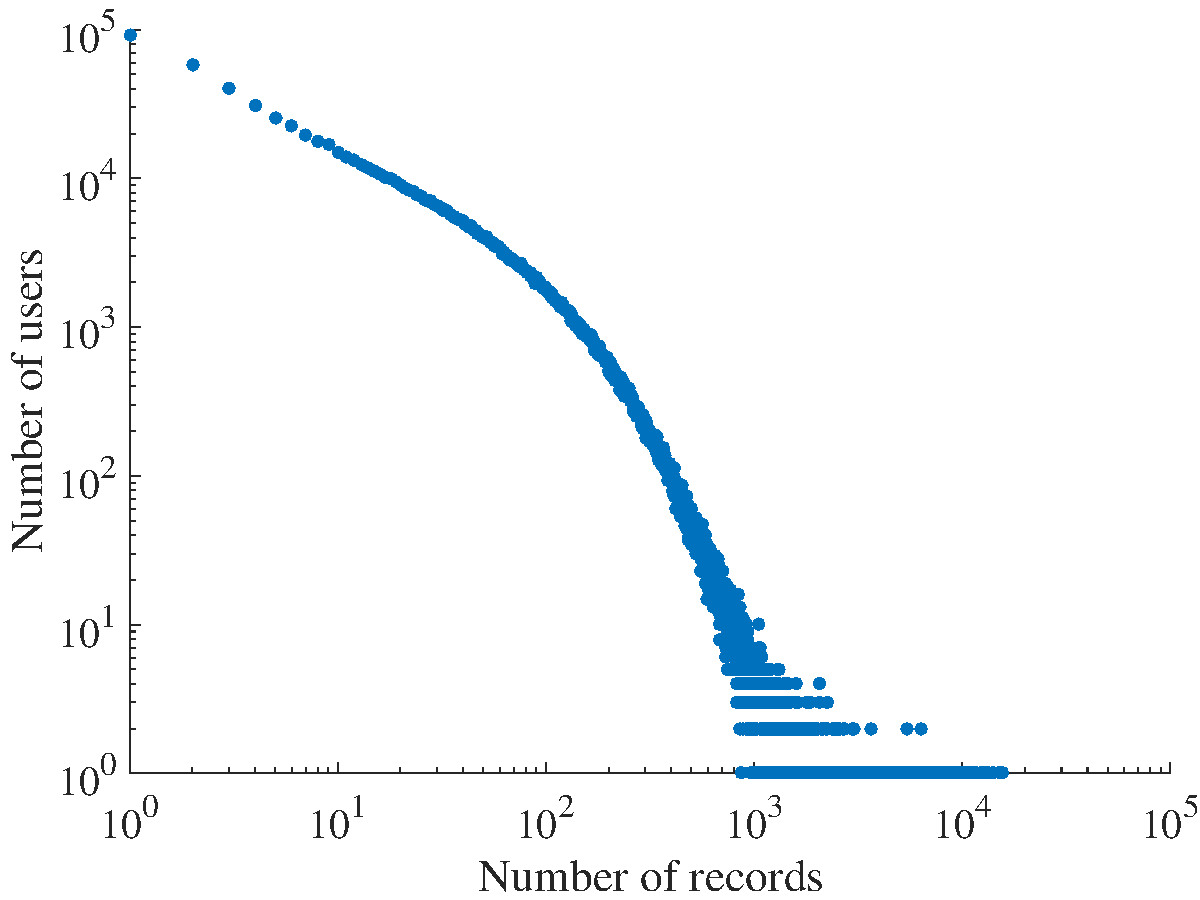
\includegraphics[width=0.32\textwidth]{figures/record_count_hist.pdf}}
  \subfigure[Avg. Time Interval      \label{fig:data_stat2}]{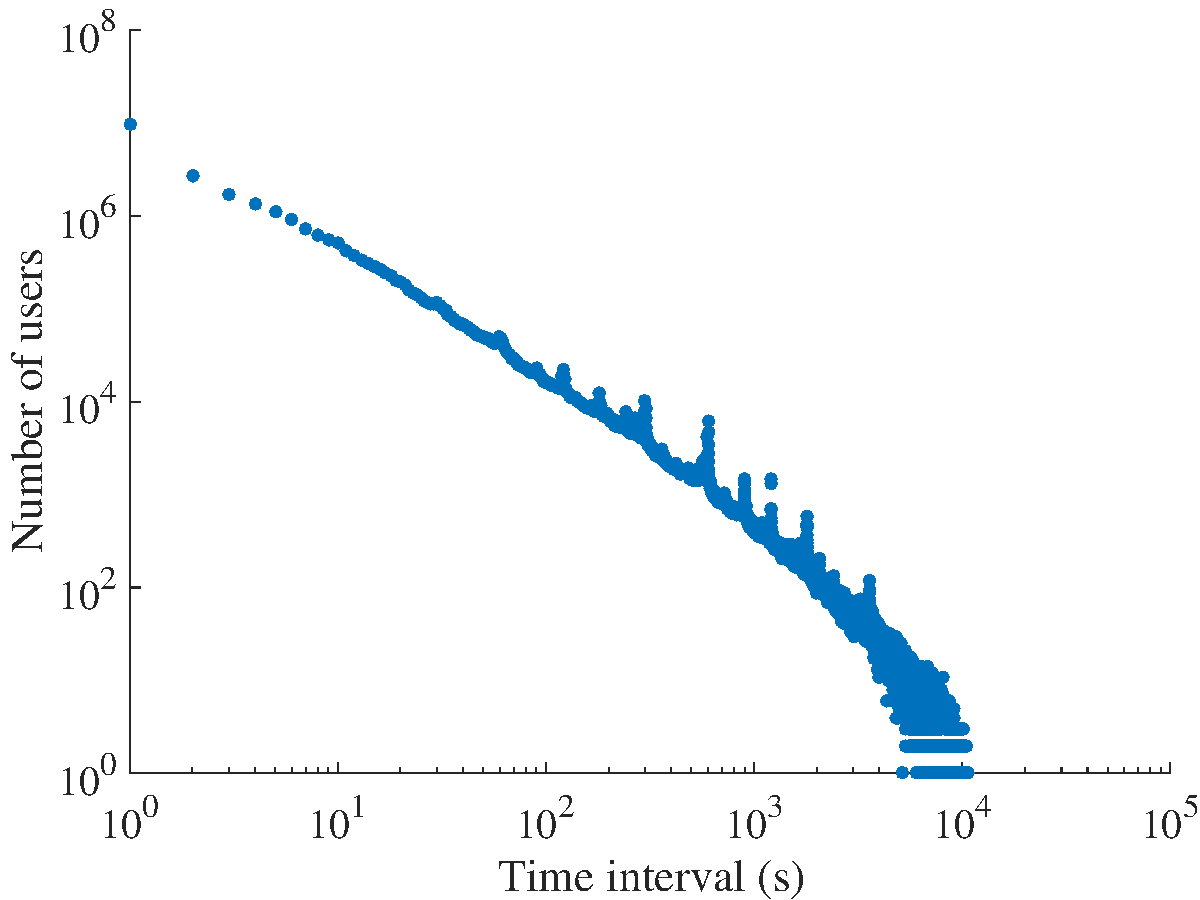
\includegraphics[width=0.32\textwidth]{figures/time_interval_hist.pdf}}
  \subfigure[Number of Towers Visited\label{fig:data_stat3}]{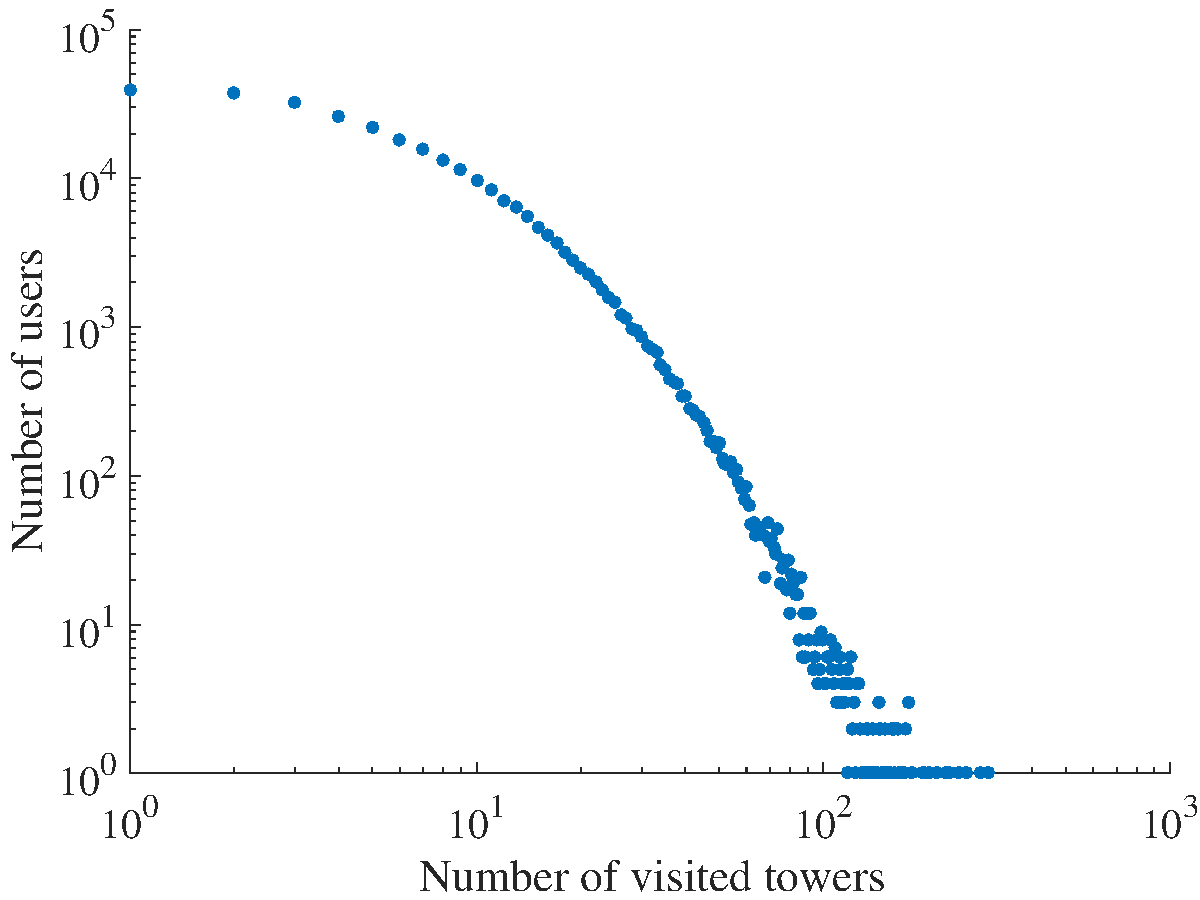
\includegraphics[width=0.32\textwidth]{figures/visited_tower_hist.pdf}}
  \vspace{-0.1in}
  \caption{Dataset characteristics.}\label{fig:data_stat}
  \vspace{-0.1in}
\end{figure*}

